% Hybrid fusion (proposed) — 가로 흐름 (왼쪽 입력 -> 오른쪽 risk). fig2_fusion_strategies (c) 를 눕히고 gate 를 더한 모양.
%   Stage 1: clinical--report arm (특징 수준 융합: l2 -> concat 128+16 -> Cox head) / image arm (CNN -> Cox head), 각자 독립 학습
%   Stage 2: r -> z 표준화 -> gated Cox combiner (g_m = 2 sigma(c_m . z), risk = sum beta_m g_m z_m), inner OOF 점수로 적합
% 점선 상자 = 독립적으로 학습되는 모델 하나 (fig2 와 같음). 빌드: tools/build_paper_figures.sh fig_hybrid_fusion
% 수치 출처: experiments/실험16_GMU_nestedCV/nested_fusion/{model.py (GatedLateFusion), config.py (FEATURE_DIMS)}.
\documentclass[tikz,border=6pt]{standalone}
% 논문 그림 공통 스타일 (fig1/fig2 가 \input 한다).
% 시각 언어는 Mixture-of-Recursions(MoR) 논문 Fig.1/2 를 따른다:
%   파스텔 채움 + 진남색 얇은 윤곽 + 둥근 모서리, 산세리프 라벨.
% 색 의미(두 그림에서 동일):
%   boxblue   = 영상 모달리티      boxpurple = 임상 모달리티     boxpink = 판독지 모달리티
%   boxgray   = 일반 연산 블록     boxyellow = Cox 관련(head/combiner)
%   dashed    = 동결(frozen) 사전학습 모듈
\usepackage[T1]{fontenc}
\usepackage{helvet}
\renewcommand{\familydefault}{\sfdefault}
\usepackage{amsmath,amssymb}
\usetikzlibrary{positioning,arrows.meta,calc,fit,backgrounds}

\definecolor{navy}{HTML}{2F3B52}
\definecolor{ink}{HTML}{1A1A1A}
\definecolor{ink2}{HTML}{5A5E66}
\definecolor{boxblue}{HTML}{CFE0F7}
\definecolor{boxpink}{HTML}{F6CDD0}
\definecolor{boxpurple}{HTML}{DCD6F3}
\definecolor{boxyellow}{HTML}{FDEEB8}
\definecolor{boxgray}{HTML}{E9E9E9}
\definecolor{cellhold}{HTML}{3F5A8A}
\definecolor{cellfit}{HTML}{F8DD8A}
\definecolor{celleval}{HTML}{F2A4A8}

\tikzset{
  every node/.style={text=ink},
  blk/.style={draw=navy, line width=0.7pt, rounded corners=2.5pt, fill=#1,
              inner xsep=4pt, inner ysep=3pt, font=\footnotesize, align=center},
  blk/.default=boxgray,
  lay/.style={blk=#1, minimum width=30mm, minimum height=6mm},
  inp/.style={blk=#1, minimum width=15mm, minimum height=7mm},
  frozen/.style={lay=boxgray, dashed},
  container/.style={draw=navy, line width=0.8pt, rounded corners=6pt, fill=white, inner sep=6pt},
  armbox/.style={draw=navy, line width=0.6pt, dashed, rounded corners=5pt, inner sep=4pt},
  arr/.style={-{Latex[length=2.2mm,width=1.7mm]}, draw=navy, line width=0.75pt},
  lab/.style={font=\scriptsize, text=ink2, align=center, inner sep=1pt},
  op/.style={circle, draw=navy, line width=0.7pt, fill=white, inner sep=0pt,
             minimum size=4.2mm, font=\scriptsize},
  risk/.style={font=\footnotesize, inner sep=2pt},
  stage/.style={font=\scriptsize\itshape, text=ink2, inner sep=1pt},
  ptitle/.style={font=\footnotesize, align=center, inner sep=2pt},
}

% ---------------------------------------------------------------------------
% 입력 모달리티 아이콘 (fig2 입력단). 글자 라벨 대신 실제 PET-CT MIP 한 장 +
% 임상 표 / 판독지 문서 픽토그램을 쓴다. 모두 약 10.5mm x 12mm 로 크기를 맞추고
% 채움색은 모달리티 색(boxblue/boxpurple/boxpink), 윤곽은 navy 로 본문 도형과 통일.
%   사용: \iconimage{노드이름}{(x,y)}  등. 노드이름으로 화살표를 걸 수 있다.
\newcommand{\iconimage}[2]{%
  \node[blk=boxblue, inner sep=1.1pt, minimum width=0pt, minimum height=0pt] (#1) at #2
       {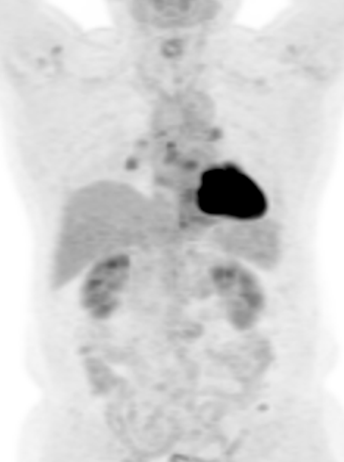
\includegraphics[height=11.8mm]{assets/pet_mip_icon.png}};%
}
\newcommand{\iconclinical}[2]{%
  \begin{scope}[shift={#2}]
    \begin{scope}
      \clip[rounded corners=2.5pt] (-5.25mm,-6mm) rectangle (5.25mm,6mm);
      \fill[boxpurple] (-5.25mm,-6mm) rectangle (5.25mm,6mm);
      \fill[navy!28]   (-5.25mm,3.3mm) rectangle (5.25mm,6mm);
      \draw[navy!45, line width=0.35pt]
        (-5.25mm,3.3mm) -- (5.25mm,3.3mm)  (-5.25mm,0.8mm) -- (5.25mm,0.8mm)
        (-5.25mm,-1.7mm) -- (5.25mm,-1.7mm) (-5.25mm,-4.2mm) -- (5.25mm,-4.2mm)
        (-1.75mm,-6mm) -- (-1.75mm,6mm)     (1.75mm,-6mm) -- (1.75mm,6mm);
    \end{scope}
    \draw[navy, line width=0.7pt, rounded corners=2.5pt] (-5.25mm,-6mm) rectangle (5.25mm,6mm);
    \node[minimum width=10.5mm, minimum height=12mm, inner sep=0pt] (#1) at (0,0) {};
  \end{scope}%
}
\newcommand{\iconreport}[2]{%
  \begin{scope}[shift={#2}]
    \fill[boxpink] (-4.6mm,-6mm) -- (-4.6mm,6mm) -- (1.7mm,6mm) -- (4.6mm,3.1mm) -- (4.6mm,-6mm) -- cycle;
    \draw[navy, line width=0.7pt, rounded corners=1pt]
      (-4.6mm,-6mm) -- (-4.6mm,6mm) -- (1.7mm,6mm) -- (4.6mm,3.1mm) -- (4.6mm,-6mm) -- cycle;
    \fill[navy!20] (1.7mm,6mm) -- (1.7mm,3.1mm) -- (4.6mm,3.1mm) -- cycle;
    \draw[navy, line width=0.55pt] (1.7mm,6mm) -- (1.7mm,3.1mm) -- (4.6mm,3.1mm);
    \draw[navy!55, line width=0.5pt]
      (-2.9mm,1.4mm) -- (2.9mm,1.4mm)  (-2.9mm,-0.4mm) -- (2.9mm,-0.4mm)
      (-2.9mm,-2.2mm) -- (2.9mm,-2.2mm) (-2.9mm,-4.0mm) -- (0.9mm,-4.0mm);
    \node[minimum width=9.2mm, minimum height=12mm, inner sep=0pt] (#1) at (0,0) {};
  \end{scope}%
}

\begin{document}
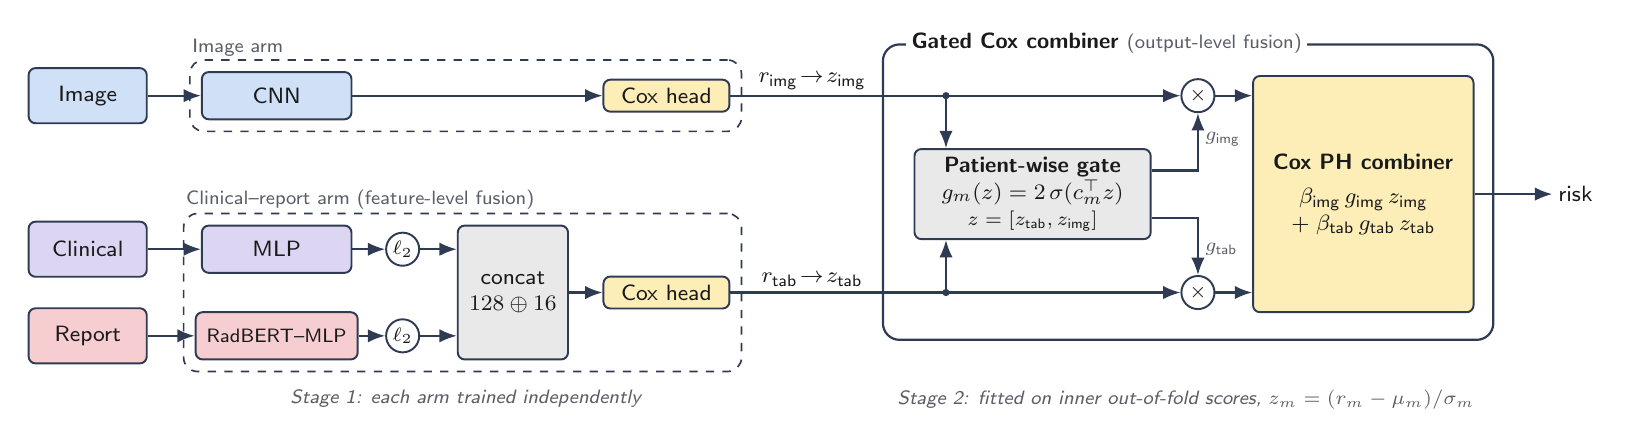
\begin{tikzpicture}[x=1cm,y=1cm]

% 행 높이: 영상 y = 2.5, 임상 y = 0.55, 판독지 y = -0.55, clinical--report 흐름 y = 0

% ===================== 입력 =====================
\node[inp=boxblue]   (xi) at (0,2.5)   {Image};
\node[inp=boxpurple] (xc) at (0,0.55)  {Clinical};
\node[inp=boxpink]   (xr) at (0,-0.55) {Report};

% ===================== Stage 1: 두 arm =====================
% image arm
\node[lay=boxblue,   minimum width=19mm] (bi) at (2.4,2.5)   {CNN};
\node[blk=boxyellow, minimum width=16mm] (hi) at (7.35,2.5)  {Cox head};
% clinical--report arm (특징 수준 융합)
\node[lay=boxpurple, minimum width=19mm] (bc) at (2.4,0.55)  {MLP};
\node[lay=boxpink,   minimum width=19mm, font=\scriptsize] (br) at (2.4,-0.55) {RadBERT--MLP};
\node[op] (lc) at (4.0,0.55)  {$\ell_2$};
\node[op] (lr) at (4.0,-0.55) {$\ell_2$};
\node[blk, minimum width=14mm, minimum height=17mm] (cat) at (5.4,0) {concat\\ $128\oplus16$};
\node[blk=boxyellow, minimum width=16mm] (ht) at (7.35,0) {Cox head};

\draw[arr] (xi) -- (bi);  \draw[arr] (xc) -- (bc);  \draw[arr] (xr) -- (br);
\draw[arr] (bc) -- (lc);  \draw[arr] (br) -- (lr);
\draw[arr] (lc.east) -- (lc.east -| cat.west);
\draw[arr] (lr.east) -- (lr.east -| cat.west);
\draw[arr] (cat) -- (ht);
\draw[arr] (bi) -- (hi);

\begin{scope}[on background layer]
  \node[armbox, fit=(bi)(hi)] (imarm) {};
  \node[armbox, fit=(bc)(br)(cat)(ht)] (tabarm) {};
\end{scope}
\node[lab, anchor=south west] at (imarm.north west)  {Image arm};
\node[lab, anchor=south west] at (tabarm.north west) {Clinical--report arm (feature-level fusion)};

% ===================== Stage 2: gated Cox combiner =====================
% 표준화된 위험점수 z 줄 위의 분기점 -> gate
\node[blk, minimum width=30mm] (gt) at (12.0,1.25)
      {\textbf{Patient-wise gate}\\ $g_m(z)=2\,\sigma(c_m^{\top}z)$\\ {\scriptsize $z=[z_{\text{tab}},z_{\text{img}}]$}};
\node[op] (mi) at (14.1,2.5) {$\times$};
\node[op] (mt) at (14.1,0)   {$\times$};
\node[blk=boxyellow, minimum width=28mm, minimum height=30mm] (cb) at (16.2,1.25)
      {\textbf{Cox PH combiner}\\[3pt] $\beta_{\text{img}}\,g_{\text{img}}\,z_{\text{img}}$\\ $+\;\beta_{\text{tab}}\,g_{\text{tab}}\,z_{\text{tab}}$};
\node[risk, anchor=west] (o) at (18.6,1.25) {risk};

% arm 출력 -> (표준화) -> 곱하기 노드
\draw[arr] (hi) -- (mi);
\draw[arr] (ht) -- (mt);
\node[risk, above] at (9.2,2.5) {$r_{\text{img}}\!\to\! z_{\text{img}}$};
\node[risk, above] at (9.2,0)   {$r_{\text{tab}}\!\to\! z_{\text{tab}}$};
% z -> gate (분기)
\coordinate (ti) at (10.9,2.5);  \coordinate (tt) at (10.9,0);
\fill[navy] (ti) circle (1.3pt);  \fill[navy] (tt) circle (1.3pt);
\draw[arr] (ti) -- (ti |- gt.north);
\draw[arr] (tt) -- (tt |- gt.south);
% gate -> 곱하기
\draw[arr] ($(gt.east)+(0,0.3)$)  -| (mi.south);
\draw[arr] ($(gt.east)+(0,-0.3)$) -| (mt.north);
\node[lab, anchor=west] at (14.15,1.95) {$g_{\text{img}}$};
\node[lab, anchor=west] at (14.15,0.55) {$g_{\text{tab}}$};
% 곱하기 -> combiner -> risk
\draw[arr] (mi.east) -- (mi.east -| cb.west);
\draw[arr] (mt.east) -- (mt.east -| cb.west);
\draw[arr] (cb.east) -- (o.west);

\begin{scope}[on background layer]
  \node[container, fit={(10.31,-0.39)(17.64,2.94)}] (gc) {};
\end{scope}
\node[font=\footnotesize, fill=white, inner sep=2pt, anchor=west] at ($(gc.north west)+(0.3,0)$)
      {\textbf{Gated Cox combiner} {\scriptsize\color{ink2}(output-level fusion)}};

% ===================== 단계 설명 =====================
\node[stage, anchor=north, align=center] at (4.8,-1.2)
      {Stage 1: each arm trained independently};
\node[stage, anchor=north, align=center] at (13.95,-1.2)
      {Stage 2: fitted on inner out-of-fold scores, $z_m=(r_m-\mu_m)/\sigma_m$};

\end{tikzpicture}
\end{document}
